\documentclass{beamer}

\usepackage{beamerthemesplit}
\usetheme{Singapore} %Copenhagen}
%\usecolortheme{whale}

%\usepackage[T2A]{fontenc}
%\usepackage[utf8]{inputenc}
%\usepackage[russian]{babel}

\usepackage[main=russian,english]{babel}   %% загружает пакет многоязыковой вёрстки
\usepackage{fontspec}      %% подготавливает загрузку шрифтов Open Type, True Type и др.
\defaultfontfeatures{Ligatures={TeX},Renderer=Basic}  %% свойства шрифтов по умолчанию
\setmainfont{Times New Roman} %% задаёт основной шрифт документа
%\usefonttheme{professionalfonts}% SOLUTION
\usefonttheme{serif}

\usepackage{hyperref}
\usepackage{textcomp}
\usepackage{amssymb,amsmath}
%\usepackage{animate}
%\usepackage{longtable}
\usepackage{xcolor}

\usepackage{pgffor}
\usepackage{enumitem}
\usepackage[export]{adjustbox}

\newcounter{N}

%% Форматирование окружения itemize
%\usepackage{ragged2e}
%\let\olditem\item
%\renewcommand\item{\olditem\justifying}

\usepackage{ mathrsfs }
\newcommand{\Rho}{\mathscr{P}}

\renewcommand{\Re}{\operatorname{Re}}
\newcommand{\Sh}{\operatorname{Sh}}
\newcommand{\Eu}{\operatorname{Eu}}
\newcommand{\Fr}{\operatorname{Fr}}

%\DeclareMathOperator{\tg}{tg}
\DeclareMathOperator{\сtg}{сtg}


\newcommand{\argxi}{(\xi^1,\xi^2,\xi^3)}
\newcommand{\argx}{(x^1,x^2,x^3)}

\newcommand{\argxiv}{(\vec{\xi})}
\newcommand{\argxv}{(\vec{x})}


\newcommand{\argxbarn}{(\bar{x}^1,\bar{x}^2,\ldots, \bar{x}^n)}
\newcommand{\argxn}{(x^1, x^2,\ldots, x^n)}

\newcommand{\argtxi}{(t, \xi^1,\xi^2,\xi^3)}
\newcommand{\argtoxi}{(t_0, \xi^1,\xi^2,\xi^3)}

\newcommand{\argtxiv}{(t, \vec{\xi})}
\newcommand{\argtoxiv}{(t_0, \vec{\xi})}


\newcommand{\argtx}{(t, x^1,x^2,x^3)}
\newcommand{\argtox}{(t_0, x^1,x^2,x^3)}

\newcommand{\argtxv}{(t, \vec{x})}
\newcommand{\argtoxv}{(t_0, \vec{x})}


\newcommand{\pd}[2]{\frac{\partial #1}{\partial #2}}
\newcommand{\pdk}[2]{\frac{\partial^2 #1}{\partial #2^2}}

\newcommand{\od}[2]{\frac{d #1}{d #2}}
\newcommand{\odk}[3]{\frac{d^{#3} #1}{d #2^{#3}}}

\newcommand{\grad}{\operatorname{grad}}
\newcommand{\rot}{\operatorname{rot}}
\newcommand{\divo}{\operatorname{div}}

\title[]{Звуковые колебания}

\author[]{ {\em Верещагин Антон Сергеевич}
\\
канд. физ.-мат. наук, старший преподаватель\\
\bigskip
Кафедра аэрофизики и газовой динамики ФФ НГУ}

\usebackgroundtemplate{
\includegraphics[width=\paperwidth]{../img/background.png}}

\begin{document}
	
\frame{\titlepage}


\frame{
	\frametitle{Аннотация}
	\parbox{\textwidth}{

	}
}

\frame{
	\frametitle{Основные уравнения динамики идеального газа}
	
	\begin{exampleblock}{Уравнения сохранения для идеального газа}
		\parbox{\textwidth}{
		\[
		\pd{\rho}{t} + (\vec{v} \cdot \nabla) \rho + \rho \divo \vec{v} = 0,
		\]
		\[
		\pd{\vec{v}}{t} + (\vec{v} \cdot \nabla) \vec{v} = -\frac{1}{\rho} \nabla p,
		\]
		\[
		\pd{S}{t} + (\vec{v} \cdot \nabla) S = 0.
		\]
			
		}
	\end{exampleblock}
	\begin{exampleblock}{Замыкающие соотношения}
		\parbox{\textwidth}{
			\[
			p = p(\rho, S).
			\]
		}
	\end{exampleblock}

}


\frame{
	\frametitle{Звуковые волны}
	
	\begin{exampleblock}{Определение}
		\parbox{\textwidth}{
			Колебательное движение с малыми амплитудами в сжимаемом газе называют \alert{звуковыми волнами}.
		}
	\end{exampleblock}\pause

	\begin{exampleblock}{Замечание}
		\parbox{\textwidth}{
			При рассмотрении звуковых колебаний будет считать течение \alert{изоэнтропическим} ($S=const$), тогда из общей системы уравнений остаются только уравнение неразрывности и уравнение Эйлера, а в замыкающем соотношении пропадает зависимость от $S$, как функции от координаты и времени.
		}
	\end{exampleblock}



	
}

\frame{
	\frametitle{Скорость звука}
		\begin{exampleblock}{Уравнения сохранения для идеального газа}
		\parbox{\textwidth}{
			\[
			\pd{\rho}{t} + \divo (\rho \vec{v}) = 0,\quad
			\pd{\vec{v}}{t} + (\vec{v} \cdot \nabla) \vec{v} = -\frac{1}{\rho} \left( \pd{p}{\rho} \right)_S \nabla \rho,
			\]
			\[
			p = p(\rho).
			\]
			
		}
	\end{exampleblock}\pause

	\begin{exampleblock}{Определение}
		\parbox{\textwidth}{
			Величина $c>0$, определяемая соотношением
			\[
			c^2 = \left( \pd{p}{\rho} \right)_S,
			\]
			называется \alert{скоростью звука}. 
			
			\medskip
			Как видно из определения $c = c(\rho, S)$. Для изоэнтропических течений зависимостью от $S$ как от функции переменных пространства и времени можно пренебречь.
		}
	\end{exampleblock}
	
}



\frame{
	\frametitle{Линеаризация уравнений движения}
	
	\begin{exampleblock}{Замена переменных}
		\parbox{\textwidth}{
			Рассмотрим малые колебания газа в окрестности постоянного решения 
			$\vec{v} = 0$, $p=p_0$, $\rho = \rho_0$:
			\[
			\begin{array}{lcl}
			\vec{v} & = & \vec{v}',\\
			c  & = & c_0 + c',\\
			\rho & = & \rho_0 + \rho '.
			\end{array}
			\]
		}
	\end{exampleblock}\pause

	\begin{exampleblock}{Уравнения движения}
		\parbox{\textwidth}{
		\[
		\pd{(\rho_0 + \rho')}{t}+ \divo(\rho_0 + \rho') \vec{v}' = 0,
		\]
		\[
		\pd{\vec{v}'}{t} + (\vec{v}' \cdot \nabla) \vec{v}' = -\frac{1}{\rho_0+\rho'} (c_0 + c')^2 \nabla (\rho_0 + \rho').
		\]
		}
	\end{exampleblock}
	
	
}

\frame{
	\frametitle{Уравнения звуковых колебаний}
	
	\begin{exampleblock}{Основные уравнения}
		\parbox{\textwidth}{
			Считая колебания малыми, отбрасываем все слагаемые, имеющие порядок малости два и выше, получим
			\[
			\pd{\rho'}{t} + \rho_0 \divo \vec{v}' = 0,\quad
			\pd{\vec{v}'}{t} + \frac{c_0^2}{\rho_0} \nabla \rho' = 0.
			\]
		}
	\end{exampleblock}\pause

	\begin{exampleblock}{Потенциальное течение и волновое уравнение}
		\parbox{\textwidth}{
			Если $\vec{v}' = \nabla \varphi$, тогда 
			\[
			\pd{\rho'}{t} + \rho_0 \Delta\varphi = 0,\quad
			\pd{}{t}\nabla\varphi + \frac{c_0^2}{\rho_0} \nabla \rho' = 0.
			\]
			\[
				\Downarrow
			\]
			\[
			\frac{1}{c_0^2} \pdk{\varphi}{t} = \Delta\varphi.
			\]
			
		}
	\end{exampleblock}
	
}

\frame{
	\frametitle{Решение волнового уравнения для плоских волн}
	
	\begin{exampleblock}{Одномерное плоское течение}
		\parbox{\textwidth}{
			Если $\varphi = \varphi(t,x)$, тогда решением полученного волнового уравнения будет
			\[
			\varphi(t,x) = f_1(x - c_0 t) + f_2(x + c_0 t) = f_1(\xi) + f_2(\eta),
			\]
			где $f_1(\xi)$, $f_2(\eta)$ -- произвольные дважды дифференцируемые функции своих аргументов
			\[
			\xi = x - c_0 t,\quad
			\eta = x + c_0 t.
			\]
		}
	\end{exampleblock}
	
}

\frame{
	\frametitle{ Прогрессивные волны }
	
	\begin{exampleblock}{}
		\centering
		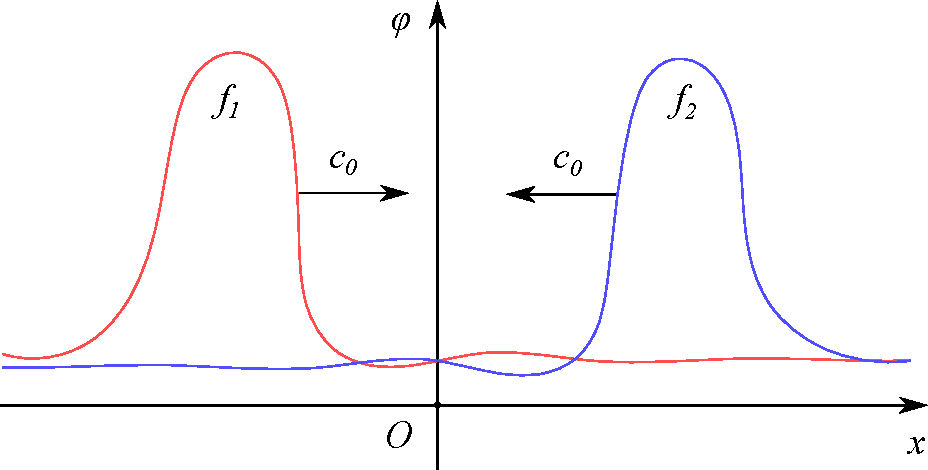
\includegraphics[width=0.9\linewidth]{../img/solitons.pdf}\\

		\parbox{\textwidth}{
			
			Решение $\varphi(t,x)$ представляет собой сумму перемещающихся поступательно вправо и влево волн неизменного вида с скоростью $c_0$.
		}
	\end{exampleblock}
}


\foreach \n in {
	01, 02, 03, 04, 05, 06, 07}
{
	
	\frame{
		\frametitle{  Иллюстрация распространения плоских волн  }
		
		\centering
		\includegraphics[width=\linewidth]{../img/solitons/signal_\n.pdf}
		
		На рисунке $\varphi(t,x) =  f_1(x - c_0 t) + f_2(x + c_0 t)$ для заданных функций $f_1(\xi)$  и $f_2(\eta)$.
	}
	
}

\frame{
	\frametitle{Решение волнового уравнения в сферической симметрии }
	
	\begin{exampleblock}{Волновое уравнение в сферической симметрии }
		\parbox{\textwidth}{
			Если $\varphi = \varphi(t,r)$, тогда волновое уравнение имеет вид
			\[
			\frac{1}{c_0^2} \pdk{\varphi}{t} = \frac{1}{r^2}
			\left(
			\pd{}{r} 
			\left(
			r^2 \pd{\varphi}{r}
			\right)
			\right)\quad
			\iff\quad
			\frac{1}{c_0^2} \pdk{}{t} (r \varphi)= \pdk{}{r}
			\left(
			r \varphi
			\right).
			\]			
		}
	\end{exampleblock}
	
	\begin{exampleblock}{Одномерное сферическое течение}
		\parbox{\textwidth}{
			Решением полученного волнового уравнения будет
			\[
			\varphi(t,r) = \frac{f_1(r - c_0 t) + f_2(r + c_0 t)}{r} = \frac{Q_1(\xi)}{r} + \frac{Q_2(\eta)}{r},
			\]
			где $Q_1(\xi)$, $Q_2(\eta)$ -- произвольные дважды дифференцируемые функции своих аргументов
			$\xi = r - c_0 t$, $\eta = r + c_0 t$.
		}
	\end{exampleblock}
	
}

\foreach \n in {05, 06, 07, 08, 09, 10, 11, 12, 13, 14}
{
	
	\frame{
		\frametitle{  Иллюстрация распространения сферических волн }
		
		\centering
		\includegraphics[width=\linewidth]{../img/solitons/spherical_signal_\n.pdf}
		
		На рисунке $\varphi(t,r) = \displaystyle\frac{1}{r}\left( f_1(r - c_0 t) + f_2(r + c_0 t)\right)$ для заданных функций $f_1(\xi)$  и $f_2(\eta)$.
		
	}
	
}


\frame{
	\frametitle{Запаздывающие потенциалы}
	
	\begin{exampleblock}{Определение}
		\parbox{\textwidth}{
			Возмущения из точки $r=0$ до доходят до некоторой точки $r \neq 0$ только через определённое время, поэтому полученное решение волнового уравнения называется \alert{запаздывающим потенциалом}.
		}
	\end{exampleblock}\pause

	\begin{exampleblock}{Потенциал источника звука}
		\parbox{\textwidth}{
			Функция вида 
			\[
			\varphi^*(t,x,y,z) = 
			-\frac{Q
				\left(
					c_0(t-t_0) - \sqrt{(x-x_0)^2 + (y-y_0)^2 + (z-z_0)^2}
				\right) 
			}
			{4\pi \sqrt{(x-x_0)^2 + (y-y_0)^2 + (z-z_0)^2} }
			\]
			является решением волнового уравнения для источника звука, начинающего действовать в момент времени $t=t_0$ в точке с координатами $(x_0, y_0, z_0)$.
		}
	\end{exampleblock}
	
}

\frame{
	\frametitle{Способы конструирования решений волнового уравнения}
	
	\begin{exampleblock}{Принцип суперпозиций}
		\parbox{\textwidth}{
			В силу линейности волнового уравнения суммарным потенциалом при движении твёрдого тела по траектории 
			\[
			x_0 = x_0(t_0),\quad
			y_0 = y_0(t_0),\quad
			z_0 = z_0(t_0)
			\]
			можно рассматривать потенциал, являющийся суммой источников звука, возбуждаемых телом в момент времени $t_0$ в соответствующих точках траектории с заданной интенсивностью $Q_{t_0}$, при этом
			\[
			\varphi = \int\limits_0^t \varphi^* dt_0.
			\]
			
		}
	\end{exampleblock}
	
}



\frame{
	\frametitle{ Литература }
	\begin{itemize}[partopsep=1pt,label=\textbullet]
		\item
%		{\em Рождественский Б.Л., Яненко Н.Н.} Системы квазилинейных уравнений и их приложения к газовой динамике. Изд. 2-е, Главная редакция физ.-мат. лит. Изд. <<Наука>>, М., 1978.
%		
%		\item
%		{\em Базаров И.П.} Термодинамика. Учеб. для вузов. -- 4-е изд., перераб. и доп. --- М.: Высш. шк., 1991. 
	\end{itemize}
}



\end{document}